\xiti
\begin{xiaotis}

\xiaoti{如图,正六棱柱的底面与投影面 $H$ 平行,它在投影面 $H$ 上的正投影是什么图形?}

\begin{figure}[htbp]
    \centering
    \begin{minipage}[b]{5.1cm}
        \centering
        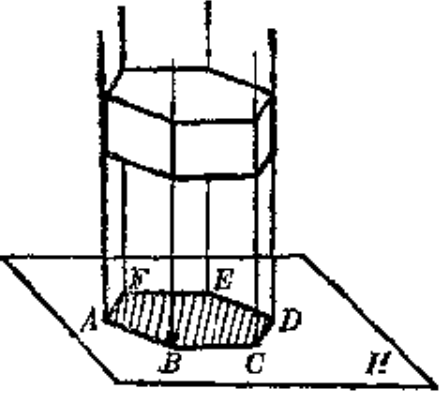
\includegraphics[width=5cm]{../pic/czjh2-ch8-xiti29-01.png}
        \caption*{(第 1 题)}
    \end{minipage}
    \qquad
    \begin{minipage}[b]{10cm}
        \centering
        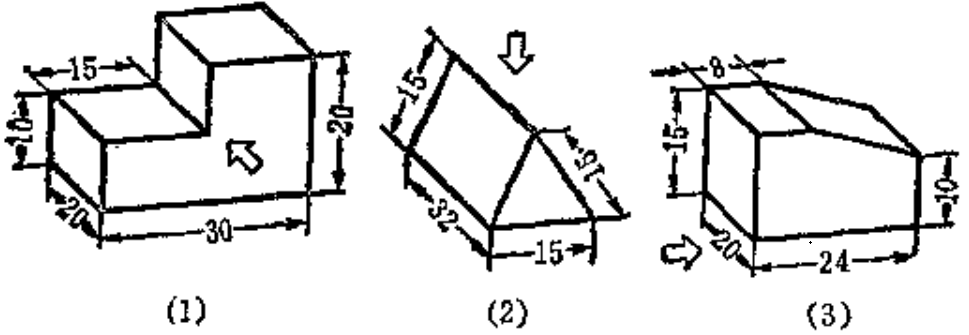
\includegraphics[width=10cm]{../pic/czjh2-ch8-xiti29-02.png}
        \caption*{(第 2 题)}
    \end{minipage}
\end{figure}

\xiaoti{画出所给几何体在指定方向的视图。\footnotemark} % 原题为“下列几何体”,因改变了图片布局。同步修改了题目
\footnotetext{本章习题中的画图题,可用铅笔画,不要求上墨。}


\xiaoti{画出底面半径为 15 mm,高为 30 mm 的圆柱的二视图。}

\begin{figure}[htbp]
    \centering
    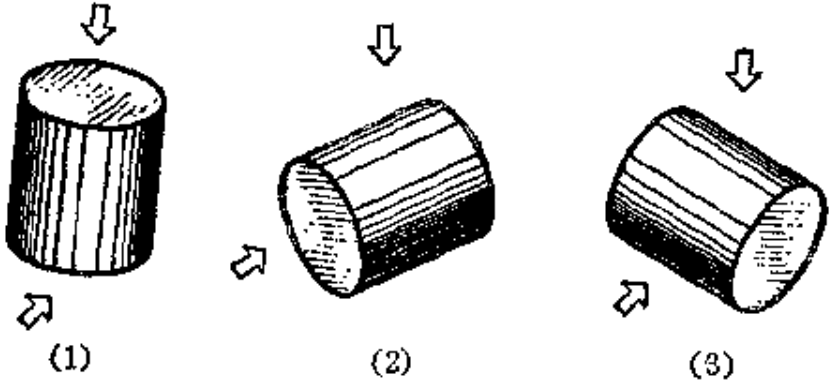
\includegraphics[width=8cm]{../pic/czjh2-ch8-xiti29-03.png}
    \caption*{(第 3 题)}
\end{figure}


\xiaoti{画出下列几何体的二视图。}

\begin{figure}[htbp]
    \centering
    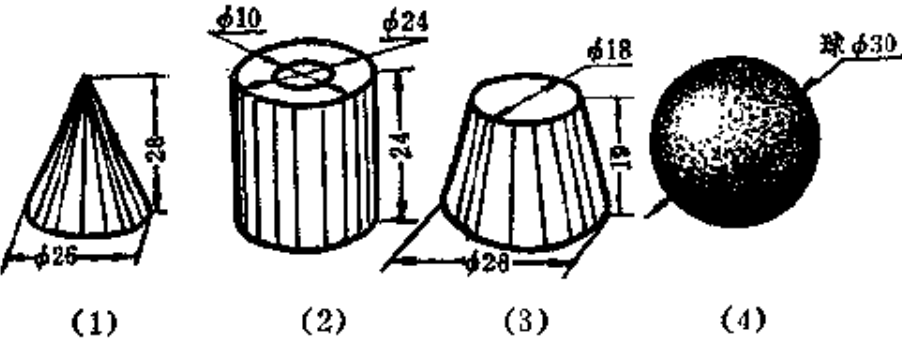
\includegraphics[width=11cm]{../pic/czjh2-ch8-xiti29-04.png}
    \caption*{(第 4 题)}
\end{figure}

\xiaoti{下列几何体的二视图有没有错误(不考虑尺寸)?为什么?如果错了,应该怎样改正?}

\begin{figure}[H]
    \centering
    \begin{minipage}[b]{4cm}
        \centering
        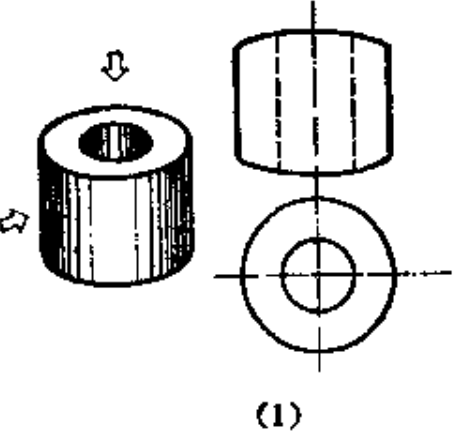
\includegraphics[width=3.5cm]{../pic/czjh2-ch8-xiti29-05-1.png}
    \end{minipage}
    \qquad
    \begin{minipage}[b]{4cm}
        \centering
        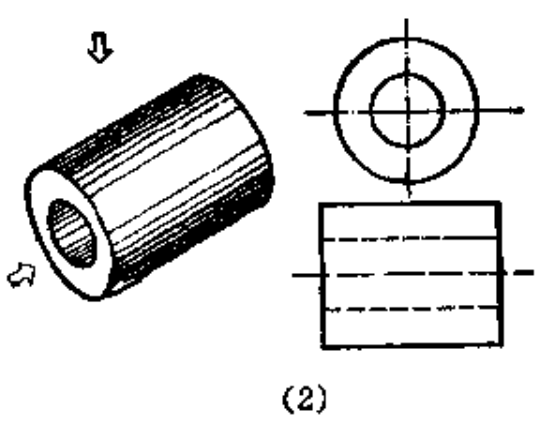
\includegraphics[width=3.8cm]{../pic/czjh2-ch8-xiti29-05-2.png}
    \end{minipage}
    \qquad
    \begin{minipage}[b]{4cm}
        \centering
        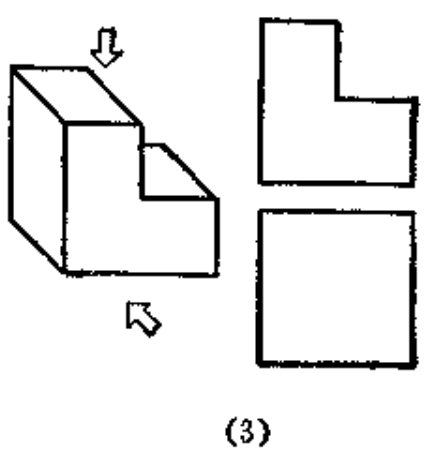
\includegraphics[width=3.3cm]{../pic/czjh2-ch8-xiti29-05-3.png}
    \end{minipage}
\end{figure} % 为了让 1、2、3 小图显示前一页,所以成两个 figure,同时指定属性 [H]

\begin{figure}[H]
    \centering
    \begin{minipage}[b]{4cm}
        \centering
        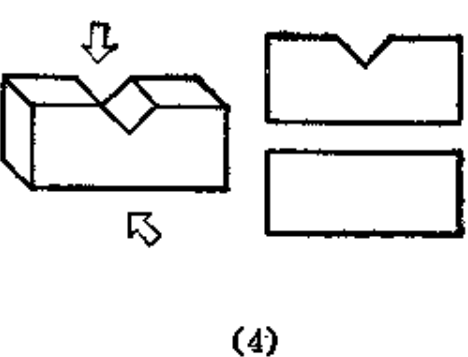
\includegraphics[width=3.8cm]{../pic/czjh2-ch8-xiti29-05-4.png}
    \end{minipage}
    \qquad
    \begin{minipage}[b]{4cm}
        \centering
        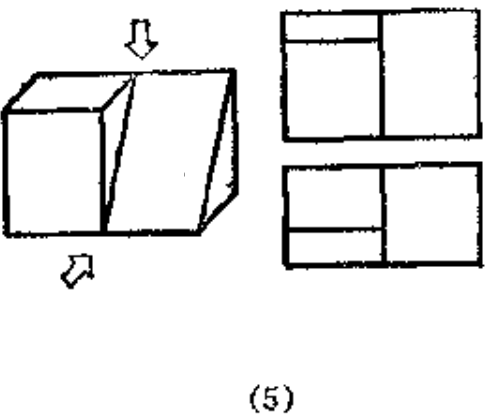
\includegraphics[width=3.5cm]{../pic/czjh2-ch8-xiti29-05-5.png}
    \end{minipage}
    \qquad
    \begin{minipage}[b]{4cm}
        \centering
        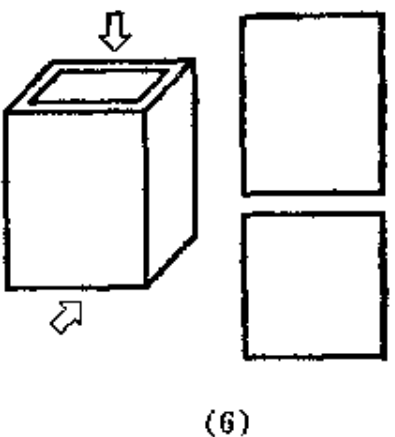
\includegraphics[width=2.8cm]{../pic/czjh2-ch8-xiti29-05-6.png}
    \end{minipage}
    \caption*{(第 5 题)}
\end{figure}

\end{xiaotis}

